\section*{Consigna}

A continuación se muestra el comportamiento de la ventana de transmisión de un cliente al subir un archivo a un servidor:

\begin{figure}[H]
    \centering
    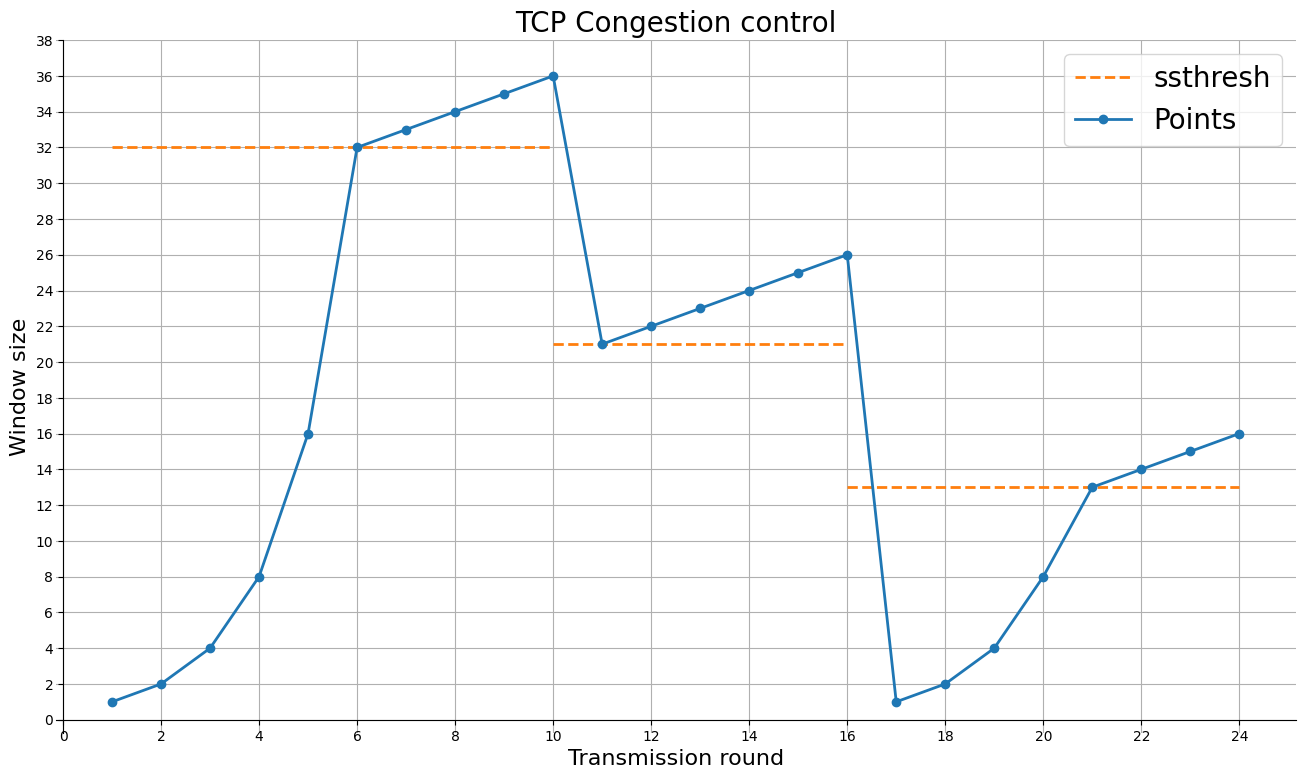
\includegraphics[width=0.95\linewidth]{Images/grafico.png}
\end{figure}

Describa el comportamiento del gráfico, mencionando el algoritmo de control de congestión utilizado, describir sus etapas, cómo se actualiza la ventana, los parámetros principales del algoritmo de congestión y el evento que causa el cambio de etapa.

\section*{Resolución}

\begin{itemize}
\item TCP Reno.
\item Slow Start.
\item Congestion avoidance.
\item Fast recovery.
\item ssthresh, cwnd.
\item Triple ACK, cada ack aumenta en uno el cwnd.
\end{itemize}



% \newpage
% \section*{Ventana}

% \subsection*{Ejercicio 1}

% Teniendo el siguiente gráfico, elija la opción correcta

% \begin{figure}[H]
%     \centering
%     \includegraphics[width=0.9\linewidth]{Images/CongestionT1.png}
% \end{figure}

% \begin{enumerate}[label=\alph*., topsep=0.5\baselineskip]
%     \item El mecanismo de control de congestión es TCP Tahoe.
%     \item Luego de la ronda de transmisión 6 ocurre un timeout.
%     \item Si después de la ronda de transmisión 15 los paquetes se reciben correctamente y ordenados, el tamaño de ventana de la ronda 18 será 32 MSS.
%     \item Luego de la ronda de transmisión 6 se reenvía un único paquete.
% \end{enumerate}


% \newpage
% \subsection*{Ejercicio 2}

% Teniendo el siguiente gráfico, elija la opción correcta

% \begin{figure}[H]
%     \centering
%     \includegraphics[width=0.9\linewidth]{Images/CongestionT2.png}
% \end{figure}

% \begin{enumerate}[label=\alph*., topsep=0.5\baselineskip]
%     \item El mecanismo de control de flujo es TCP Reno.
%     \item Luego de la ronda de transmisión 5 ocurre un timeout.
%     \item Si después de la ronda de transmisión 15 los paquetes se reciben correctamente y ordenados, el tamaño de ventana de  la ronda 16 será 16 MSS.
%     \item Luego de la ronda de transmisión 5 se reenvía un único paquete.
% \end{enumerate}
